\documentclass[11pt]{article}

\usepackage{fancyhdr}
\usepackage{amsmath}
\usepackage{tikz}
\usepackage{pgfplots}
\pgfplotsset{compat=1.18}

\pagestyle{fancy}
\fancyhead[L]{AP Calculus BC}
\fancyhead[R]{1.4 Parametric Equations}
\fancyfoot[C]{\thepage}

\newcommand{\emptygraph}{
    \begin{center}
    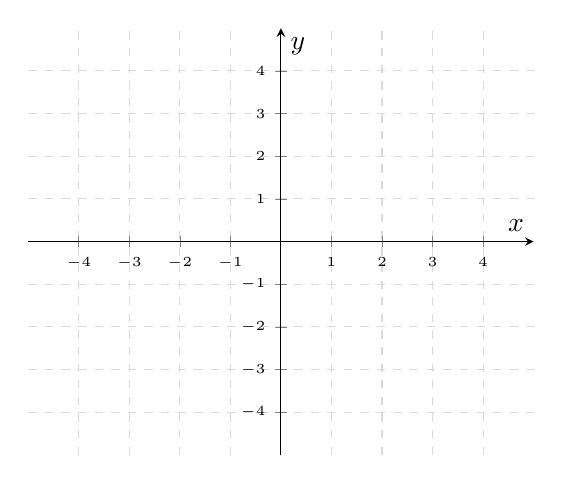
\begin{tikzpicture}
        \begin{axis}[
            axis lines = middle,
            grid = both,
            width=8cm,
            height=7cm,
            xmin=-5, xmax=5,
            ymin=-5, ymax=5,
            xtick={-4,-3,...,4},
            ytick={-4,-3,...,4},
            xlabel={$x$},
            ylabel={$y$},
            tick label style={font=\tiny},
            grid style={dashed, gray!30}
        ]
        \end{axis}
    \end{tikzpicture}
    \end{center}
}

\begin{document}

\noindent And now for something completely different: parametric equations. Why? The best way to understand is to look at something in motion:

\vspace{1cm}

\noindent We can describe motion in a coordinate plane, but we cannot also show the time of motion. To do that, we introduce a third variable, $t$, called a parameter. Bad news: this is challenging. Good news: we can use our calculator.

\vspace{1cm}

\noindent Describe the graph of the relation determined by $x = \sqrt{t}, y = t, t \ge 0$. Indicate the direction in which the curve is traced and find the Cartesian equation.

\emptygraph

\noindent Notice how important domain is\dots we call the domain $I$ the parameter interval.

\vspace{0.5cm}

\noindent \textbf{Definition:} If $x$ and $y$ are given as functions $x = f(t), y = g(t)$ over an interval of $t$-values, then the set of points $(x,y) = (f(t), g(t))$ defined by these equations is a \textbf{parametric curve}. The equations are \textbf{parametric equations} for the curve.

\newpage

\noindent Also notice that direction matters\dots the parameter $t$ determines where the curve starts and ends. Describe the graph of the relation determined by the following. Determine initial and terminal points and determine the Cartesian equation.

\[x = 2\cos{t}, y = 2\sin{t}, 0 \le t \le 2\pi\]

\emptygraph

\noindent Again, graph the parametric curve: $x = 3\cos{t}, y = 4\sin{t}, 0 \le t \le 2\pi$

\emptygraph

\newpage

\noindent At this point, you might think that parametric equations are used primarily for graphs of conics. However, we can also graph a line segment. Draw and identify the graph of the parametric curve: $x = 3t, y=2 - 2t, 0 \le t \le 1$

\emptygraph

\noindent Find a parameterization for the line segment with endpoints $(-2,1)$ and $(3,5)$.

\vspace{4cm}

\end{document}
